\chapter{Grid Storage Strategies}                \label{sec:grid-implementations}

In this section, we explain different approaches for storing into memory the regular and unstructured grids which will be used by the stencil computations in subsequent sections. We detail considerations that need to be made when choosing memory layouts for grids for the CUDA platform.

As indicated in section \ref{sec:grids}, we will use the two notions of coordinates in Euclidean space and indices (=addresses) in memory in the following to describe how grids are stored. Two aspects of a grid and its storage implementation need to be described:
\begin{enumerate}
    \item The way the \emph{values} stored inside a cell are laid out in memory, i.e. how coordinates in Euclidean space map to indices in memory.
    \item How the \emph{neighborship relations} for a cell are defined, i.e. given a certain cell, how to find the desired neighbor.
\end{enumerate}

\section{Regular Grids}

Both indexing and neighborship relations are easy to determine in regular grids. Thanks to the grid's regularity, coordinates in combination with the dimension of the grid carry enough information to be directly translated to memory locations.

\subsection{Row-major Indexing}

The coordinates can directly be mapped to a memory index by simple arithmetic. The perhaps most popular way to do this is \emph{row-major indexing}. This is the memory layout many programming languages such as \emph{C} use to lay out multi-dimensional arrays in memory. The cells of the grid are indexed as follows: A cell at coordinates $p$ receives the offset
 $$\text{index}\left(p_x, p_y, p_z\right) = p_x + p_y \cdot d_x + p_z \cdot d_x \cdot d_y.$$
Herein, the factors besides the coordinates are called the strides, i.e. the \emph{x-stride} is $1$, \emph{y-stride} is $d_x$ and \emph{z-stride} is $d_x\cdot d_y$. Only in a regular grid are the strides constant -- this is the advantage of using a regular grid. Stepping through the memory linearly, this means that the X-coordinate is the fastest-changing and the Z-coordinate is the slowest-changing. Using this scheme, memory locality is good for cells with similar X-coordinates, but not necessarily so for cells with similar Y- or Z-coordinates.

\subsection{Neighborship Relations}

With row-major indexing, in order to access the value of a neighbor of a cell at position $p$, it suffices to know the coordinates of the cell and the strides of the grid. The indices of the left (right), top (bottom), and front (back) neighbors are simply given by subtracting (adding) the x-stride, y-stride, or z-stride respectively. This gives the same index as subtracting one from (adding one to) the respective X-, Y- or Z-coordinate and then calculating the index as described above. All that is required for accessing a neighbor's value is simple arithmetic for the index and a memory load at the calculated index to receive the cell's stored value.

For example, in memory, the left neighbor of a cell in memory at location $i$ is located at $i-1$ the top neighbor at $i-1\cdot d_x$ and the back neighbor (Z-dimension) is at $i-1\cdot d_x\cdot d_y$. From this, it is evident that when using row-major indexing in regular grids, neighbors in the X-dimension (left/right) will have great memory locality. However, as the grid dimension in X- or Y-dimension exceeds beyond what the processor can hold in the cache, accesses to neighbors in Y- or Z-direction become more costly. 

\subsection{Memory Alignment}

\label{sec:regular-memory-alignment}
The Cuda compiler generally ensures that data structures are well-aligned in memory for the target architecture for coalescing accesses. However, when storing a regular grid for later stencil applications, manual alignment calculations can become necessary due to the \emph{halo} (as defined in section \ref{sec:halo}). 

Consider some stencil applied to a regular grid. Because of the lack of neighboring values, a kernel will not operate on values at the boundary of the grid, the halo. The first thread actually executing any load/store instructions will be on an inner value. Therefore, if the halo is not a multiple of the vector load instruction size (32), some loads at the beginning and end of each row will not be aligned. The addresses of the halo cells are not loaded and thus wasted in the instruction.

This problem can be aleviated by adding paddings such that not the first \emph{inner} value is 32-byte-aligned instead of the very first element of the array. Given a halo of size $h = \begin{pmatrix}h_x & h_y & h_z\end{pmatrix}^\top$ we want the cell at coordinate $h$ to be aligned, not $\begin{pmatrix} 0 & 0 & 0\end{pmatrix}^\top$. We thus chose minimal paddings $a$, $b$ and $c$ and reformulate the index computation such that
\begin{gather}
    \text{index}\left(p_x, p_y, p_z\right) = p_x + a + p_y \cdot \left(d_x + b\right) + p_z \cdot \left(d_x \cdot d_y + c\right) \label{eq:regular-index}
    \\
    \text{index}\left(h_x, p_y, p_z\right) \equiv 0 \mod 32 \qquad \text{for all $p_y$, $p_z$}
\end{gather}

Note that the modulo computations are only performed upon grid generation (on the CPU). Once the grid is stored in memory, stencils require only the chosen paddings $a, b, c$ as additional inputs in order to correctly compute the memory index of a cell at any coordinate (according to equation \ref{eq:regular-index})

\section{Unstructured Grids}

In completely unstructured grids, 
memory indices are in no fixed relation to coordinates. This complicates neighbor accesses. Adjacency information for each cell must be explicitly stored. Accessing a given cell's neighbors requires a lookup of this information. This is contrary to regular grids, where adjacency information is implicitly known through coordinates and grid dimensions (i.e. constant strides).

To facilitate some optimizations and more accurately model the typical unstructured grids in meteorological applications, we restrict the notion of an unstructured grid throughout the remainder of this thesis. Specifically, we pose the following requirements to our unstructured grid implementation and stencils operating on it:

\begin{enumerate}
    \item \textbf{Regular in Z-dimension:} The grid remains regular in the Z-dimension, i.e. the mentioned decoupling of indices and coordinates only occurs in the X-Y-plane. For neighbors in the X-Y-plane, cells with equal X and Y coordinates have the same relative neighborship offsets at all Z-levels. The Z-coordinate retains its meaning and can be used in conjunction with the Z-stride $d_xd_y$ to access neighbors in the Z-dimension. Conversely, the Z-coordinate of a cell can be inferred from the cell's index $i$, specifically $p_z = i \mod d_xd_y$. Note that knowledge of the absolute Z-coordinate is not required in stencil code, thus costly modulo operations never occur in stencil code.
    \item \textbf{Stencils operate only on a bounded region, relative to each cell:} A stencil operating on some cell requires only its own cell's fields, its neighbor's fields up to some bounded depth $l$ and constant inputs to calculate its results. Only relative offsets to the current cell's coordinates are accessed. Stencils applied on our unstructured grid do not require knowledge of absolute X and Y coordinates. Given a cell at memory index $i$, determining its coordinates $p_x, p_y$ is \emph{not} required in stencil (GPU) code. (Of course, the mapping is defined and must be accessible in CPU code in order to access and display the grid values -- this access is not required to be efficient, though.) 
\end{enumerate}

As with the regular grid, our implementation must define how the \emph{values} (next section) and the \emph{neighborship information} (section \ref{sec:unstructured-neighborships}) are stored. We describe certain important considerations in the context of a SIMT application for both but focus on the latter.

\subsection{Memory Layout and Indexing of Cells} 
\label{sec:unstructured-indexing}

The inner values in our unstructured grid implementation may be stored in an arbitrary layout. The \emph{halo} cells must be stored separately from the inner values. In this separate block of halo cells, the memory layout may also be arbitrary. In the following subsection, we describe the considerations that were made in the context of halo storage.

While completely arbitrary layouts for the values are possible, some patterns of regularity will be present in most real-world use cases. Section \ref{sec:emulating} describes the two types of memory layouts (\emph{row-major}, \emph{z-curves}) we simulated when benchmarking our unstructured grid implementation.

\subsubsection{Halo}

To ensure correct results, stencils may only operate on cells where the required neighbors for the output calculation are present. In the regular case, this is ensured by checking in each thread that the current coordinate lies within the inner part of the grid or within the halo. In regular grids, this is fast: coordinates can be determined from memory indices using only arithmetic. On the other hand, a thread in our unstructured grid implementations can not know the absolute coordinate of a cell it operates on, due to the possibly arbitrary layout of cells and unknown (to the thread) mapping from indices to coordinates. For unstructured implementations, a thread receives only a memory address of some cell, for which it must compute the result. Therefore, another approach must be taken.

One solution works as follows: The required neighborship lookups are performed in every thread. When the desired neighbor is not present, a special value indicates this; the program concludes at this point that the currently being operated-on cell lies in the halo and aborts. This might happen, for example, when a thread operating on the topmost cell asks for the index of the cell above it. Consider a neighborship storage implementation that stores a relative offset of the index for each neighbor; in this type of implementation, an offset of $0$ is effectively a pointer to the same address/cell the thread is already operating on. It could, therefore, be used as a special value to indicate the required neighbor is not present.

There are two main disadvantages to this approach: First, even for cells in the halo, a (possibly costly) memory lookup is performed before threads determine no computation can be done. Second, due to the inactive/aborted halo-threads, there will be under-utilized memory loads, similar to uncoalesced accesses. The considerations for coalescing made in section \ref{sec:regular-memory-alignment} for regular grids do not apply here, because in an unstructured grid with varying strides no constant padding can be chosen to ensure coalescing accesses. 

A better solution is to store the halo and inner values in separate blocks in memory. Threads are then initiated to only operate on the inner value block. We opted to store any cell located in the halo of the stencil in front of any of the inner values in memory. With this approach, we can safely operate threads on the memory block of only inner values and be sure to never encounter a halo cell. If there are several stencils with different-sized halos to be applied to the same unstructured grid, spiralling storage of the halo cells moving from the outwards in can even be employed. The starting address of the first inner value then determines what is considered as inner value by the stencil. Stencils with a smaller halo can operate on a memory block starting at a lower address, including some cells that would lie in another stencil's halo. However, storing the halo at the beginning, separated from inner values, comes at the cost of a reduced memory locality for inner cells whose neighbors reside in the halo. This cannot be avoided.

Across all of our implementations, we employed the second approach of storing the halo separately, in front of the inner values. As in the benchmarks, only one stencil was applied to each grid at once, we did not use the spiraling scheme; halo cells are simply stored in a row-major fashion, followed by the inner values.

\subsection{Neighborship Relations}
\label{sec:unstructured-neighborships}

To characterize an unstructured grid, adjacency information about all cells must be explicitly stored in memory. We store this information in what we call \emph{neighborship tables}.  For clarity, we will refer to two distinct blocks of memory in the following: The \emph{neighborship block} stores information about the structure of the grid, while the \emph{data block} stores the values of the cells.

Suppose there are $m$ types of \emph{neighborship relations} (e.g. top, bottom, left and right neighbors, $m=4$), i.e. each cell can have at most $m$ neighbors. For each relation, one array of size $d_xd_y$ is allocated in the neighborship block. Each array functions as the \emph{neighborship table} for one relation (e.g. a top-, bottom-, left- and right-array). Consider a cell whose value is stored in an array at index $i$ in the data block. In each neighborship table, at offset $i \mod d_xd_y$, a pointer to a neighbor of that cell is stored. This pointer is a relative offset from the index $i$.

Storing relative offsets instead of absolute pointers has the advantage that a thread working on the value at index $i$ does not need to know where the beginning of the data block is; it can simply add the offset to the index. An offset of $0$ signifies that the cell at this index does not have such a neighbor.

The described neighborship tables are akin to adjacency lists\cite[Chapter 12]{DSA}. Consider a graph representation of a grid, where nodes represent cells, and edges represent the neighborship of two cells. Given $m$ types of neighborship relationships (e.g. ``top'', ``bottom'', ``left'' and ``right''), we create $m$ such graphs linking the respective neighbors (e.g. a graph connecting all nodes with their ``upper'' neighbor). Each neighborship table is the adjacency list of such a graph, where the cells are referred to by their relative offset from the current cell in memory. 

All neighborship tables are stored consecutively in memory. We allocate $\mathtt{sizeof(int)}\cdot m \cdot d_x d_y$ bytes in the neighborship block to store the neighborship tables. A pointer to the $k$-th neighbor of a cell stored at index $i$ can be found in the $k$-th neighborship table at index $i \mod d_xd_y$. Herein, the modulo $d_xd_y$, i.e. the Z-stride, is required for memory indices $i$ for $Z>0$ to remove the Z-component from the index.

Putting all of this together, the following equation \ref{eq:unstr-neigh} describes how the index (in the data block) of the $k$-th neighbor in the X-Y-plane of a cell stored at index $i$ (in the data block) is computed. The ordering (i.e. which neighbor is the $k$-th) can be defined arbitrarily, as long as it remains consistent.

\begin{gather}
    \text{neighbor}_k(i) = i + \mathtt{neigh[}d_xd_y\cdot k + (i \mod d_xd_y)\mathtt{]} \label{eq:unstr-neigh}
\end{gather}

Herein, the function $\text{neighbor}_k(i)$ gives the index of the $k$-th neighbor of the input cell, $\mathtt{neigh}[l]$ refers to the $l$-th element in the neighborship block (as in C), and $d_xd_y$ is the Z-stride (i.e. dimensions of the X-Y-plane). Note that modulo calculations are expensive operations; our optimized grid access variants (see section \ref{sec:optimizations}) thus avoid those by using the three dimensions of the thread index to give an index in the X-Y-plane (which would be the result of the modulo operation) and the Z-coordinate separately. Further note that thanks to the regularity in the Z-dimension, neighbors in the Z-direction can be accessed without an additional lookup by simple addition or subtraction of the Z-stride, $d_xd_y$.

\textit{Example:} Given an array \texttt{values} representing the data block, which stores the values of each cell, an array \texttt{neighbors} representing the neighborship block, and assuming the ``right'' neighborship relation is defined as the 2nd ($k=2$) in the neighborship block, then the value of the right neighbor of cell $i$ is stored at $\mathtt{values[}i + \mathtt{neighbors[}2\cdot d_xd_y(i \mod d_xd_y)\mathtt{]]}$.

The stencils benchmarked in section \ref{sec:results} are defined in terms of regular grids. In our implementations, we limit each cell to have at most $4$ directly adjacent neighbors. This is the maximum number of neighbors any cell in a two-dimensional quadrilateral grid can have.

The described neighborship storage approach can be further optimized. In the  benchmarks in section \ref{sec:results}, we will present four variations for the described neighborship tables, resulting from the combination of two properties:

\begin{itemize}
    \item \emph{Chasing / non-chasing}
    \begin{itemize}
        \item \emph{Chasing}: Adjacency information is stored only for direct neighbors. Accessing neighbors-of-neighbors requires pointer chasing.
        \item \emph{Non-chasing}: Adjacency information is stored up to some depth $l$ (as required by the stencil). One lookup suffices to determine the index of a neighbors-of-neighbors, but additional memory for the neighborship table is required.
    \end{itemize}
    \item \emph{Uncompressed / compressed}
    \begin{itemize}
        \item \emph{Uncompressed}: The neighborship table contains one entry for each cell in the X-Y-plane.
        \item \emph{Compressed}: Cells with the same relative neighborship offsets share their neighborship table entries. An additional lookup (akin to a dictionary mapping cells to their neighborship table entries) is required.
    \end{itemize}
\end{itemize}

Given a grid with four neighborship types ($m=4$), representing the entire grid's values and its structure, including neighbors-of-neighbors up to depth $l \geq 1$, can be achieved with a memory footprint of 
$$\mathtt{sizeof(int)} \cdot d_xd_y \cdot 2 l(l+1) + \mathtt{sizeof(T)}\cdot d_xd_yd_z \quad \text{bytes}$$
Herein, \texttt{T} is the data type used for values (\texttt{float} or \texttt{double}, or a struct for array-of-struct-type storage of multiple fields, see \ref{sec:representing-multiple-fields}).

\subsubsection{Coalescing of neighborship lookups}

Storing neighborship offsets in multiple separate arrays in the described manner is crucial for on-GPU execution. It enables coalescing of the accesses to the neighborship tables. Suppose some stencil computation, in which multiple threads desire to calculate the output value for several cells at consecutive memory addresses. They will all require access to the same neighboring cells at each computation step (as the exact same stencil computation is applied to every cell). Therefore, if, for example, all threads require the top neighbor, consecutive addresses in the top-neighbor table will be requested and accesses will get coalesced. If, however, we had a ``classical'' adjacency list, where the top, bottom, left and right neighbors were each stored together (intertwined) for every cell, accesses by threads to the top-neighbor would be separated by a stride of four elements (the other neighbors), thus making coalescing impossible and forcing sequential loads. The two approaches to storing multiple neighborships are also referred to as \emph{array-of-structs} and \emph{struct-of-arrays}, and are further discussed in section \ref{sec:representing-multiple-fields}, where the analogous problem for storing multiple values (fields) per cell is addressed.

\subsubsection{Pointer Chasing}

Some stencils will require neighboring cells beyond directly adjacent ones, i.e. neighbors-of-neighbors up to a certain depth $l$. As described above, an entry in the neighborship table is stored only for each neighborship \emph{relation}. Accessing the neighbor of a neighbor thus requires so-called \emph{pointer chasing}: Two lookups to the neighborship tables in series, where the second lookup location is determined by the result of the first. Due to this dependency, such lookups cannot be performed in parallel.

To avoid the issue of \emph{pointer chasing} it can be beneficial to store all neighbors-of-neighbors up to a certain depth $l$ in additional neighborship tables. This increases the memory footprint but can enable faster access to neighbors-of-neighbors.

In a grid where each cell is limited to four direct neighbors, storing all neighbors and neighbors-of-neighbors up to a depth of $l$ requires $2\cdot l(l+1)$ pointers per cell in the X-Y-plane.

\subsubsection{Compression} \label{sec:compression}

In unstructured grids with some regular components, the neighborship tables contain many redundant entries. In a regular subsection of the grid, the relative offsets of the neighbors' indices are identical. We thus consider a  compression scheme for the neighborship tables. Even though memory limits are not a constraint for any of the benchmarked stencils, compression is interesting for performance (runtime) reasons. This is due to caching; when many threads access the same neighborship table entries, it is very likely those entries reside in the cache and are available much more quickly. Several cells sharing the same neighborship table entries also leaves more room in the cache for entries for other cells.

Yet, to be beneficial to performance, a compression scheme must be very lightweight. Any computation required for decompression adds to the total runtime and could cancel out or even outweigh the described caching advantages. The following proposed scheme was able to provide some benefit for large enough grids (see section \ref{sec:results}). % TODO more specific reference

\paragraph{Compression phase}

The compression phase occurs on the CPU, upon grid generation. Consider a completely regular grid stored in row-major order. Except for the halo cells, the relative neighbor index offsets are equal to the X- and Y-strides for every cell. In principle, only one neighborship table entry per neighborship relation would thus suffice to encode the strides. In unstructured grids, multiple of these \emph{patterns} of neighborship relations may occur if there are regular components. Our compression works by grouping together such patterns of neighbor index offsets. 

The structure of the grid is described by neighborship offsets $o = (o_1, \dots, o_m)$ for each cell. Each of the $m$ offsets describes the relative offset of one of the neighborship relations. In the compression phase, we create a new pattern for each unique vector of offsets $o$ encountered. The offsets for each pattern are stored \emph{exactly once} in the neighborship tables. All offsets for one pattern reside at the same pattern index in the neighborship tables. An additional array $\mathtt{pattern}$ of size $d_xd_y$ is allocated. This array provides a mapping from each cell (cell index) to its corresponding pattern (i.e. the index in the neighborship tables).

\paragraph{Stencil phase}

During the stencil computation, a thread operating on a cell with index $i$ looks up the pattern of its neighborships by reading $\mathtt{pattern[}i \mod d_xd_y\mathtt{]}$. (The optimized access strategies seperate the X-Y-component in the index $i$ from the Z-coordinate and as such do not require the modulo computation in their actual implementation.) For any subsequent neighborship lookup, the neighbor pointers are read from the neighborship tables using the previously obtained index from the pattern array. The previously described equation \ref{eq:unstr-neigh} for neighborship access is altered to the following:

\begin{gather}
    \text{neighbor}_k(i) = i + \underbrace{\mathtt{neigh[}d_xd_y\cdot k + \overbrace{\mathtt{pattern[}(i \mod d_xd_y)\mathtt{]}}^\text{pattern lookup}\mathtt{]}}_\text{(hopefully cached) neighbor lookup} \label{eq:unstr-neigh-comp}
\end{gather}

Compare this to the uncompressed variant: there, the initial lookup of patterns is skipped, and neighborship tables are accessed at $i\mod d_xd_y$. In the uncompressed case, each entry in the neighborship table is only relevant to one cell, and only accessed by one thread per Z-level. In contrast, if compression is effective, there will be relatively few patterns, and the same few neighborship table entries will be accessed by many threads. We anticipate that those few neighborship table entries will reside in the caches due to their large number of accesses. We note that compression adds one indirect lookup (pointer chasing through the pattern array). For this scheme to be effective at reducing the runtime, the positive effect due to caching of the second lookup must outweigh the cost of the required additional pattern lookup.

It appears to be unavoidable to have the $d_xd_y$-sized pattern array if the complete flexibility of an unstructured grid is to be retained. But, thanks to compression, this should most likely be the only array whose entries are solely relevant to one cell per Z-level; neighborship table accesses should concentrate around a few relevant entries.

\paragraph{Using Constant Memory} For uncompressed neighborship accesses, coalescing accesses can be easily attained because the access pattern is known beforehand. In the compressed case, the accesses depend on the result of the pattern lookup. Multiple threads often access the same neighborship table entries. This is not optimal for coalescing. For broadcast-type accesses, i.e. when all threads access the same address, constant memory is better suited. Constant memory provides broadcasting capabilities, but its separate L1 cache is smaller in the Volta architecture. We experimented with storing the neighborship tables in constant memory. The pattern array remained in regular global memory, as the coalescing problems do not apply there (every thread accesses its own entry, no interference). While, for the very regular grids with an exact row-major layout, this yielded a small speedup around $5\%$, it turned out to be much slower for more varied data layouts, such as a \emph{z-order} curves layout (slowdown around $15\%$). Because the latter is much more realistic in a real-world unstructured grid use case, we opted not to use constant memory in our final implementation of compression. Table \ref{tab:constmem} shows the effects of using constant memory on one exemplary stencil.

\begin{table}
    \comment{./gridbenchmark --no-verify --size 512x512x64 --threads 256x1x1 laplap-unstr-idxvar -z laplap-unstr-idxvar -z -c laplap-unstr-idxvar -z -c --cmem laplap-unstr-idxvar laplap-unstr-idxvar -c laplap-unstr-idxvar -c --cmem 
Benchmark                           , Precision, Domain size,,, Blocks     ,,, Threads    ,,, Kernel-only execution time                
                                    ,          ,   X,   Y,   Z,   X,   Y,   Z, 
                                      X,   Y,   Z,   Average,    Median,   Minimum,   Maximum
laplap-unstr-idxvar                 ,    double, 512, 512,  64,   2, 508,  64, 256,   1,   1,    813752,    814280,    807060,    817870
laplap-unstr-idxvar-comp            ,    double, 512, 512,  64,   2, 508,  64, 256,   1,   1,    553346,    553390,    548490,    559230
laplap-unstr-idxvar-cmem-comp       ,    double, 512, 512,  64,   2, 508,  64, 256,   1,   1,    523820,    523600,    519830,    528120
laplap-unstr-idxvar-z-curves-4      ,    double, 512, 512,  64,   2, 508,  64, 256,   1,   1,    778175,    778990,    771070,    785390
laplap-unstr-idxvar-comp-z-curves-4 ,    double, 512, 512,  64,   2, 508,  64, 256,   1,   1,    562292,    561945,    557220,    570630
laplap-unstr-idxvar-cmem-comp-z-curves-4,    double, 512, 512,  64,   2, 508,  64, 256,   1,   1,    638830,    638870,    633790,    643250}
	
	\begin{center}
    \begin{tabular}{l l l l}
        \hline \hline 
        \textbf{Storage} & \textbf{Compression} & \textbf{Constant Memory} & \textbf{Runtime} \\
        \hline
        row-major & - & - & $814\mu s$ \\
        row-major & \checkmark & - & $553\mu s$ \\
        row-major & \checkmark & \checkmark & $\mathbf{524\mu s}$ \\
        \hline
        z-curves & - & - & $770\mu s$ \\
        z-curves & \checkmark & - & $\mathbf{562\mu s}$ \\
        z-curves & \checkmark & \checkmark & $639\mu s$ \\
        \hline \hline
    \end{tabular}
	\end{center}
    \caption{\label{tab:constmem} Effect of using constant memory applying the \emph{Laplace-of-Laplace} stencil on a $512\times 512\times 64$-sized grid with $256\times 1\times 1$ threads. Using constant memory gives a slight $5\%$ advantage in the highly regular row-major grids; for the more realistic z-curve scenario, it results in a slowdown of $14\%$.}
\end{table}

\subsection{Indirect Addressing Overhead} \label{sec:emulating}

In our benchmarks (see section \ref{sec:results}), we compared the performance of stencils on regular vs. unstructured grids. To ensure a fair comparison, it was important to be able to produce and verify the exact same output for both the regular and the unstructured grids. This was only possible by ``emulating'' an unstructured grid; we took the regular grid as a base, and then also represented it as if it were an unstructured grid, i.e. created a neighborhsip table for it and used indirect addressing in the stencils. This enabled us to capture the overhead of indirect addressing with otherwise unchanging conditions. Note that even though we benchmarked a grid with completely regular neighborships in the unstructured case, this knowledge was not made use of in the optimizations of the unstructured grid -- as they stand, the implemented programs would also support completely arbitrary unstructured grids in two dimensions.

In these emulated unstructured grids (essentially regular grids using indirect addressing), we stored the same values as in the regular grid using two layouts: \emph{row-major} (as in the regular grid case) and a variation of Z-order curves (referred to in the remainder of this thesis in short as \emph{z-curves}). Note that the Z in ``Z-order curves'' refers to the shape described by this memory layout, not to the Z-dimension of our grid. We only use the described memory layouts to store two-dimensional planar slices of our grid.

The memory layout of the emulated unstructured grid using a row-major layout is almost identical to the one for regular grids. The only difference lies in the different handling of the halo values, which is done as described in section \ref{sec:unstructured-indexing}. 

\begin{figure}
	\begin{center}
    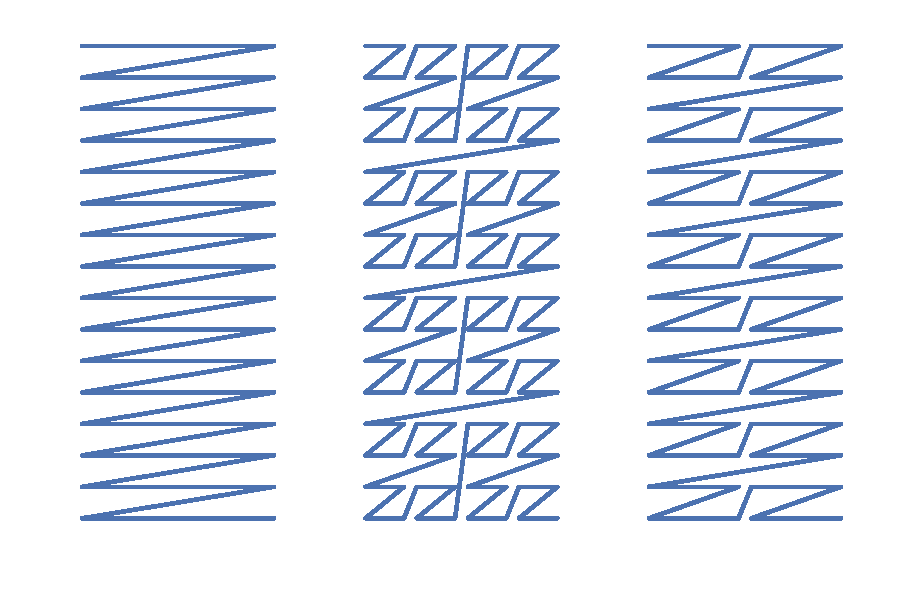
\includegraphics[width=\textwidth]{layouts.pdf}
	\end{center}
    \caption{\label{fig:layouts} The different memory layouts described. The blue lines illustrate the order in which the cells in the X-Y-plane of the grid are stored in memory. The lowest memory index always starts at the top-left corner. Left: Row-major indexing. Middle: Normal z-order curve. Right: Widened z-order curve.}
\end{figure}

Z-order curves\cite{wiki:z-curves} represent a more realistic unstructured scenario. A variation of this layout might be used to represent a true unstructured grid with some irregularities. The aim of Z-order curves is to give most cells with close X-, Y- and Z-coordinates close indices. Locality is achieved by \emph{intertwining} the bits of the X- and Y-components of a coordinate, starting with the X-coordinate at the least-significant bit. The middle graph in figure \ref{fig:layouts} shows a Z-order curve. Observe how the blue line representing the order of memory indices seldom makes large jumps, meaning points that are close in physical space remain close in memory. Compared to the row-major layout (left in that figure), this is a big improvement in locality.

Consider a two-dimensional coordinate, wherein both components are given as a bit string of even length $n$ as:
$$p=\begin{pmatrix}p_x & p_y\end{pmatrix}^\top=\begin{pmatrix}\left\langle p_x^{(n)} p_x^{(n-1)} \cdots p_x^{(2)} p_x^{(1)} \right\rangle & \left\langle p_y^{(n)} p_y^{(n-1)} \cdots p_y^{(2)} p_y^{(1)} \right\rangle\end{pmatrix}^\top$$
The index in Z-order curve ordering is then given by:
\begin{gather}
    i = \left\langle p_y^{(n)} p_x^{(n)} p_y^{(n-1)} p_y^{(n-1)} \cdots p_y^{(2)} p_x^{(2)} p_y^{(1)} p_x^{(1)}\right\rangle
\end{gather}

In this thesis, we have implemented a memory layout which uses a modified Z-curve layout in the X-Y-plane. To make use of CUDA's vector instructions, which can consume up to 32 bytes of consecutive memory at once when properly aligned, the Z-curve implemented is a stretched out variant. The last five bits are \emph{not} intertwined. To ensure the indices are dense, the cells are then ordered by the number obtained due to this intertwining way and are indexed in a consecutive manner from lowest to highest intertwined number.

Using this, we get repeated lines of 32 cells that share their relative neighborship offsets with other such lines; this allows better-coalesced accesses. Using a width of 32 ensures that coalescing is possible even for one-byte data types; when using four- or eight-byte floating-point types, the width could be reduced. We briefly experimented with smaller stretchings of the Z-curve and observed only minimal differences in runtimes. In the z-curves layout, neighborship offsets are more varied than in a row-major layout, rendering both compression and coalescing less efficient. This is thus a more realistic and useful scenario for modeling a real unstructured grid.

Using a truly arbitrary, randomized memory layout was also considered, but not pursued further after initial tests. In grids with a randomized layout, cache locality was completely destroyed, leading to runtimes around eight times the row-major or z-curve variants. For example, the \emph{Laplace-of-Laplace} stencil described in section \ref{sec:results} completed in around $814 \mu s$ for a row-major layout, whereas it took $6999 \mu s$ in a completely random layout in otherwise identical conditions. However, such a completely random memory layout is highly unrealistic. Even in real unstructured meteorology applications, large portions of the grid would remain regular. Unstructuredness only occurs in boundary areas, e.g. between areas of different resolutions. Evaluating the performance implications of a completely random layout provide little value to the implementation of meteorological stencils and possible optimizations would be very limited.


\section{Representing Multiple Fields} \label{sec:representing-multiple-fields}

Two of the three benchmarked stencils and most real-world applications perform calculations that require more than one input value per cell in the grid. There are two obvious approaches to storing multiple \emph{fields} for both regular and unstructured grids, \emph{array-of-structs} and \emph{struct-of-arrays}.

\paragraph{Array of Structs}
In the array-of-structs memory layout, all fields for one cell are stored together, before any values for the next cell. This means that accesses to different fields of the same cell have good memory locality, whereas accessing the same field of different cells requires larger strides.

\paragraph{Struct of Arrays}
In the struct-of-arrays layout, there are $k$ arrays for $k$ fields. This is conceptually the same as having $k$ different one-field grids. Different fields of the same cell are stored in separate arrays and are thus separated by (at least) the size of one array. This approach requires additional care to keep the indices for cells synchronized across all arrays; deleting or adding a cell requires access to all $k$ arrays.

The struct-of-arrays approach is highly beneficial to most GPU stencil implementations because of coalescing. When a stencil is implemented such that each thread is responsible for the calculation of one output value, all threads will most likely try to access the same field on different cells concurrently. In the struct-of-array layout, these accesses are able to coalesce (if the cells appear consecutively in memory).  Because of this, we have implemented all our benchmarks in this fashion, i.e. as multiple one-field grids. To verify the claim that array-of-structs is slower than struct-of-arrays, we have implemented both variants for the \emph{fast waves} benchmark, see table \ref{tab:array-of-structs}.

\begin{table}
	\begin{center}
    \begin{tabular}{l c c}
        \hline
        \textbf{Benchmark} & \textbf{Run Time} & \textbf{Load Efficiency} \\
        \hline
        \hline
        Array of Structs & $8282 \mu s$ & $25.73\%$\\
        Struct of Arrays & $2546 \mu s$ & $99.39\%$ \\
        \hline
    \end{tabular}
	\end{center}
    \caption{\label{tab:array-of-structs} Comparison of run times and global load efficiency (ratio of requested loads to performed loads, where bad coalescing leads to more loads being performed than needed) for the fast waves benchmark with domain size $512\times 512\times 64$ and block size of $128\times 1\times 2$.}
\end{table}

However, in the struct-of-arrays approach, cache locality might suffer from the large strides between the fields of a cell. It might be desirable to also load the other fields of a cell into the cache when one field of that cell is accessed. In this approach, however, only identical fields from other cells are close and thus loaded in the cache. A compromise that seeks to combine both the caching advantages of array-of-structs and the coalescing of struct-of-arrays is the \emph{array-of-structs-of-arrays} approach, which stores one array, which for each warp-sized block of cells contains a struct of warp-sized arrays for each field. We have not implemented this.
